\documentclass{ltxdoc}

\def\fileversion{0.1}
\def\filedate{2017/09/05}

\title{The \textsf{limecv} document class\thanks{This document corresponds to \textsf{limecv}~\fileversion, dated \filedate.}}

\author{Olivier Pieters \\ \texttt{me (at) olivierpieters (dot) be}}

\usepackage{listings}
\usepackage{tikz}
\usepackage{hyperref}

\usepackage{cleveref}
\usepackage{xparse}

\lstset{%
  basicstyle=\ttfamily, % font style and size
  breakatwhitespace=false,
  breaklines=true,
  numbers=left,
  numberstyle=\tiny,
  numbersep=5pt,
  language=[LaTeX]{TeX},
  keywordstyle=\color{blue},
  commentstyle=\color{red}
}

\NewDocumentCommand{\cvRequirement}{m}{\textbf{#1}}

\begin{document}

\maketitle

\section{Introduction}

This document class is designed to facilitate easy development of curriculum vit\ae\ (CV) with this particular design. Special elements have been designed of particular sections to ease quick creation. This document class was co-designed with a business card, which can be found on GitHub: \url{https://github.com/opieters/business-card}.

The design of this CV is split up in three parts, illustated by \cref{design}. Each of these parts that make up this CV template, will be detailed in the sections below.

\begin{figure}[!ht]
  \centering
  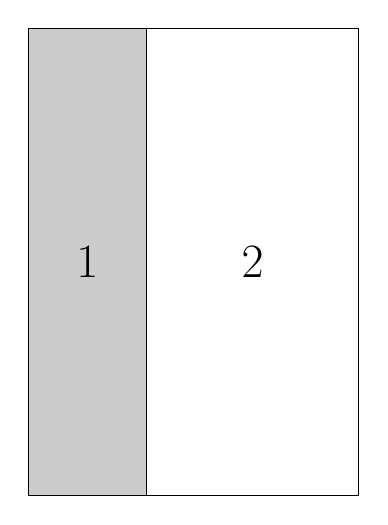
\begin{tikzpicture}
    \draw (0,0) rectangle ++(4.20,5.94);
    \draw[fill=black!20] (0,0) rectangle ++(1.5,5.94);
    \draw (0.75,2.97) node {\LARGE 1};
    \draw (2.85,2.97) node {\LARGE 2};
  \end{tikzpicture}%
  \hspace{2cm}%
  
\begin{tikzpicture}
    \draw (0,0) rectangle ++(-4.20,-5.94);
    \draw[fill=black!20] (0,0) rectangle ++(-4.2,-1.5);
  \end{tikzpicture}
  \caption{Illustation of basic template. The left image depicts the actual CV: side bar to the left (1) with main content on the right (2). The right image depicts the cover letter design.}
  \label{design}
\end{figure}

\section{Requirements}

  Currently, it is advised to use the \cvRequirement{XeLaTeX} compiler. LaTeX will also work, but in that case icons are not available. In the subsequent, it will always be assumed that the XeLaTeX compiler is used (unless noted otherwise). 

  Any font can be used, though by default the \cvRequirement{Fira}\footnote{\url{https://github.com/mozilla/Fira}} font is used. This should be installed and accessable by the typesetting system. If another font is desired, it can be overwritten using the \lstinline|customfont| document class options and |\cvMainFont| command. 

  \cvRequirement{FontAwesome}\footnote{\url{http://fontawesome.io}} is the icon font used. This font should also be available and cannot be replaced by another icon font. 

\section{General Macros and Document Class Options}

\section{Side Bar}

  The side bar should contain personal information such as your name, job title (or industry or similar), contact information, small bio, interests and language skills. Special environments and commands have been defined for each of these sections and will be described below. 

  Everything that should be inside the side bar should be placed in the |cvSideBar| environment. This environment is placed on the left side of the page by default. If it should be typeset on the right side, use the starred version (|cvSideBar*|)

  The following environments are available inside the side bar environment: |cvProfile|, |cvContact|, |cvLanguages|, |cvInterests| and |cvProjects|.
  
  \DescribeMacro{\cvID}
  This command typesets a picture (in a circle) with name and position underneath it.
  The argument order is: |\cvID{|\meta{first name}|}{|\meta{last name}|}{|\meta{picture location}|}{|\meta{job position}|}|. Empty fields are allowed for the third and fourth arguments. No picture and no job position will then be typeset. Example code: 
  \begin{lstlisting}
\cvID{John}{Doe}{profile_picture}{Broaker}
  \end{lstlisting}
  
  \DescribeMacro{cvProfile} 
  This environment contains a brief profile description or biography. No additional arguments are allowed. Example code:
  \begin{lstlisting}
\begin{cvProfile}
  A short biography goes here.
\end{cvProfile}
  \end{lstlisting}
  
  \DescribeMacro{cvContact} 
  All the contact information goes here. Inside this environment, the following commands are available: 
  \begin{itemize}
    \item \DescribeMacro{\cvContactAddress} |\cvContactAddress{|\meta{address}|}| typesets an address. How this address should be typeset exactly is left to the user. The use of line breaks (|\\|) is allowed;
    \item \DescribeMacro{\cvContactEmail} |\cvContactEmail{|\meta{link}|}{|\meta{email address}|}| typesets an email address. The link variable should be a something like |mailto:john@doe.tld|. Clicking on the email address will then automatically open the default email client with this address as recipient. If the link argument is left empty, no link will be created. 
    \item \DescribeMacro{\cvContactPhone} |\cvContactPhone{|\meta{mobile phone number}|}| typesets a mobile phone number.
    \item \DescribeMacro{\cvContactWebsite} |\cvContactWebsite{|\meta{link}|}{|\meta{website URL}|}| typesets a website. The link variable should be a something like |https://johndoe.tld|. Clicking on the website will then automatically open the default web browser. If the link argument is left empty, no action will be performed upon clicking on the website.
    \item \DescribeMacro{\cvContactGithub} |\cvContactGithub{|\meta{link}|}{|\meta{username}|}| typesets a GitHub profile. The link variable should be a valid link to the GitHub profile (for example |https://github.com/johndoe|). Clicking on the username will then automatically open the default web browser. If the link argument is left empty, no action will be performed upon clicking on the website.
    \item \DescribeMacro{\cvContactLinkedin} |\cvContactLinkedin{|\meta{link}|}{|\meta{username}|}| typesets a LinkedIn profile. The link variable should be a link to your LinkedIn profile homepage (for example |https://www.linkedin.com/in/johndoe/|). Clicking on the username will then automatically open the default web browser. If the link argument is left empty, no action will be performed upon clicking on the website. 
    \item \DescribeMacro{\cvContactTwitter} |\cvContactTwitter{|\meta{link}|}{|\meta{username}|}| typesets a Twitter profile. The link variable should direct to your Twitter profile. An example link looks as follows: |https://twitter.com/johndoe|. Clicking on the username will then automatically open the default web browser. If the link argument is left empty, no action will be performed upon clicking on the website.this address as recipient. If the link argument is left empty, no link will be created. 
    \item \DescribeMacro{\cvContactKeybase} |\cvContactKeybase{|\meta{link}|}{|\meta{fingerprint}|}| typesets a keybase fingerprint (and account). The link variable should be a link to the KeyBase profile (e.g.\ |https://keybase.io/johndoe|). Clicking on the fingerprint will then automatically open the default web browser. If the link argument is left empty, no action will be performed upon clicking on the website.
  \end{itemize}
  
  A full example:
  \begin{lstlisting}
\begin{cvContact}
  \cvContactAddress{Some Street 78\\B-9000 Ghent\\Belgium}
  \cvContactEmail{mailto:john@doe.tld}{john@doe.tld}
  \cvContactPhone{+1 781 555 1212}
  \cvContactWebsite{https://doe.tld}{doe.tld}
  \cvContactGithub{https://github.com/johndoe}{johndoe}
  \cvContactLinkedin{https://www.linkedin.com/in/johndoe/}{johndoe}
  \cvContactTwitter{https://twitter.com/johndoe}{@johndoe}
  \cvContactKeybase{https://keybase.io/johndoe}{\texttt{AAAA 5555 BBBB FFFF}}
\end{cvContact}
  \end{lstlisting}

  If you wish to add contact information that is not available by default, you can extend the command using two internal commands: |\cv@ContactTemplateLink| and |\cv@ContactTemplate|. See the source code for usage instructions.

  \DescribeMacro{cvLanguages} This environment is used to showcase language skills. The \DescribeMacro{\cvLanguage} |\cvLanguage{|\meta{language}|}{|\meta{skill level}|}| should be used inside this environment. The skill level is a real value with a maximum value of 5. If higher values are used, the result will not be typeset properly. An example is included below.

  \begin{lstlisting}
\begin{cvLanguages}
  \cvLanguage{English (native)}{5}
  \cvLanguage{German (B1)}{3}
  \cvLanguage{Spanish}{3}
\end{cvLanguages}  
  \end{lstlisting}

  \DescribeMacro{cvInterests} Typeset interests (can be both professional and personal) using |cvInterests|. By default it just typesets a list of items in the long format (|long|). The short format can be activated by passing the |short| option to the environment. Inside this environment, three commands can be used: |\cvInterestsPersonal|, |\cvInterestsProfessional| and |\cvInterest|. \DescribeMacro{\cvInterestsPersonal} |\cvInterestsPersonal| and \DescribeMacro{\cvInterestsProfessional} |\cvInterestsProfessional| add optional sections inside this environment to differentiate between personal and professional interests respectively. Both macros have no options nor arguments. The \DescribeMacro{\cvInterest} |\cvInterest{|\meta{icon}|}{|\meta{interest}|}| command takes an icon and interest as arguments. Note that if \LaTeX\ is used, the icon argument will be ignored. In this case, there is also no difference between the |long| and |short| options of the |cvInterests| environment.
  
  Examples that illustrate the different options are depicted below:

  \begin{lstlisting}
\begin{cvInterests}
  \cvInterestsPersonal
  \cvInterest{\faTrain}{model trains}
  \cvInterest{\faFlask}{(applied) sciences}
  \cvInterest{\faSuitcase}{travelling}
  \cvInterestsProfessional
  \cvInterest{\faGraduationCap}{machine learning}
  \cvInterest{\faMicrochip}{electronics}
  \cvInterest{\faCogs}{robotics}
\end{cvInterests}
  \end{lstlisting}
  
  \begin{lstlisting}
\begin{cvInterests}[short]
  \cvInterestsPersonal
  \cvInterest{\faTrain}{model trains}
  \cvInterest{\faFlask}{(applied) sciences}
  \cvInterest{\faSuitcase}{travelling}
  \cvInterest{\faCamera}{photography}
  \cvInterest{\faGamepad}{gaming}
  \cvInterest{\faMusic}{music}
\end{cvInterests}
  \end{lstlisting}
  
  \DescribeMacro{cvProjects} If you have interesting (side) projects that are relevant for your CV, you can list them using the |cvProjects| environment. Inside this environment you can use the \DescribeMacro{\cvProject} |\cvProject[|\meta{options}|]{|\meta{name}|}{|\meta{description}|}| macro to list all your projects. The only options currently allowed in \meta{options} are to pass an image (using |image|) and a URL (using |link|). This image must be an external file and the user must handle its size through |width| or |height|. Example usage:
  
  \begin{lstlisting}
\begin{cvProjects}
  \cvProject[image=clock,width=1cm]{yanic}{An IoT nixie clock.}
  \cvProject{\texttt{limecv}}{A \LaTeX\ document class for curriculum vit\ae.}
\end{cvProjects}
  \end{lstlisting}
  
  It is currently not possible to extend the side bar with additional environments. To add your own, look at the source code and create your own \LaTeX-style hack.  

\section{Main Section}

\section{Cover Letter}

\section{Example}

  The source code of a typical CV document can be found below. \Cref{example-cv,example-cover-letter} depict the resulting PDF documents.

  \begin{figure}[!ht]
    \includegraphics[width=\textwidth,page=1]{mwe.pdf}
    \caption{Example CV (scaled).}
    \label{example-cv}
  \end{figure}

  \begin{figure}[!ht]
    \includegraphics[width=\textwidth,page=2]{mwe.pdf}
    \caption{Example cover letter (scaled).}
    \label{example-cover-letter}
  \end{figure}

  \lstinputlisting[language=tex]{mwe.tex}

\section{Source Code}

\lstinputlisting[language=tex]{limecv.cls}

\end{document}